\documentclass[12 pt]{article}
\pagestyle{empty}
\addtolength{\topmargin}{-0.9in}
\addtolength{\textheight}{1.9in}
\addtolength{\oddsidemargin}{-0.7in}
\addtolength{\textwidth}{1.4in}
\newcommand{\D}{\displaystyle}
\usepackage{amsmath, tikz}

\begin{document}
  \begin{center}
    \textbf{\hfill MATH 040 -- Week 9 homework} \\
  \end{center}
  \medskip

  \noindent
  \textbf{Name}\ \rule{3.5in}{.4pt} \hfill
  \vspace{.1in}
  \hspace*{0.2in}

	\medskip
  \noindent

  \begin{enumerate}
    \item Simplify the following exponential expressions.
    \begin{enumerate}
      \item $54^0 = $
      \\
      \item $(14^{-1})^{-1} = $
      \\
      \item $9^{-2} = $
      \\ \vspace{1.5cm}
      \item $\displaystyle\frac{3^7\cdot5^2}{(3^2)^3 \cdot 5 \cdot 5^2} = $
      \\ \vspace{1.5cm}
      \item $\displaystyle \frac{2^15 - 2^7}{(2^2)^3} = $
      \\ \vspace{1.5cm}
      \item $\displaystyle\frac{2^8}{(2^{-3})^{-2}} = $
      \\ \vspace{1.5cm}
      % \item Graph the function.\\
      % \begin{tikzpicture}[scale = 1.2]
      %   \draw (-4,-4) grid (4,4);
      %   \draw[ultra thick, <->] (-4.2,0)--(4.2,0);
      %   \draw[ultra thick, <->] (0,-4.2)--(0,4.2);
      %   \node at (4.4,0) {$x$};
      %   \node at (0,4.4) {$y$};
      % \end{tikzpicture}
      \item $(x^3x^{-1})^{-2} = $\\ \vspace{1.5cm}
      \item $\displaystyle\frac{xy^8}{(y^{-3})^{-2}} = $
      \\ \vspace{1.5cm}
    \end{enumerate}
		\pagebreak
		\item
      Write the following in scientific notation: \begin{enumerate}
        \item $7.2 \cdot 10 \cdot 10 \cdot 10 \cdot 10$
        \\ \vspace{2cm}
        \item $6 + 2\cdot 10^2$
        \\ \vspace{2cm}
        \item The number of grains of sand on earth is $7\,500\,000\,000\,000\,000\,000$.
        \\ \vspace{2cm}
        \item The number of atoms in a grain of sand is $43$ quintillion.
        \\ \vspace{2cm}
        \item The number of atoms in \textit{all} of the sand on earth.
        \\ \vspace{2cm}
        \item $(2.5 \cdot 10^5) \cdot (8 \cdot 10^{-1})$
        \\ \vspace{2cm}
        \item $\displaystyle \frac{3.6 \times 10^8 + 4 \times 10^7}{2 \times 10^3}$
      \end{enumerate}
      \pagebreak
    \item In class last week, we estimated the weight of all of the water in Lake Superior. In this problem, we'll estimate the weight of the moon.
    \begin{enumerate}
      \item Using telescopes, we can estimate that the diameter of the moon is about 2000 miles. Using the information that the radius is half of the diameter, and that the volume of a sphere is $\frac 43 \pi r^3$, what is the \textit{volume} of the moon in cubic miles and scientific notation? (Round to two decimal places.)
      \\ \vspace{3cm}
      \item Using the information that $1$ mile is equal to $1600$ meters, what is the volume of the moon in $\text{m}^3$ (and scientific notation)? \\
      (Recall that if $\displaystyle 1 = \frac{1600 \text{m}}{1 \text{mi}}$, then $\displaystyle 1^3 = 1 = \left(\frac{1600 \text{m}}{1 \text{mi}}\right)^3 = \frac{1600^3 \text{m}^3}{1 \text{mi}^3}.$)
      \\ \vspace{3cm}
      \item Using that $1\text{m}^3$ weighs $2200$ pounds, how much does the moon weigh in pounds?
      \\ \vspace{3cm}
      \item Using that $1\text{m}^3$ weighs $2200$ pounds, how much does the moon weigh in pounds?
      \\ \vspace{3cm}
      \item The Pacific Ocean contains $1.5 \cdot 10^{21}$ pounds of water. The moon weighs how many more times than the Pacific Ocean?
    \end{enumerate}
    \pagebreak
    \item Determine whether each of the functions are polynomials. If a function is a polynomial, find the degree.
    \begin{enumerate}
      \item $f_1(x) = -3x^5 -\frac{2}{3}x^2 + \sqrt{71}$
      \\ \vspace{1cm}
      \item $f_2(x) = -x^{-5} -7x^{-2} + 7$
      \\ \vspace{1cm}
      \item $f_3(x) = x^4 + 3^x - 7x^2 + x + 1$
      \\ \vspace{1cm}
      \item $f_4(x) = x(x+1)(x+2)(x+3)$ \hfill \textit{(What are the roots?)}
      \\ \vspace{1cm}
      \item $f_5(x) = x^2 - 100$ \hfill \textit{(What are the roots?)}
      \\ \vspace{1cm}
      \item $f_6(x) = x(x+1)(x+2)(x+3)(x^2 - 100)$ \hfill \textit{(What are the roots?)}
      \\ \vspace{1cm}
    \end{enumerate}
    \item Use a calculator or website that can graph functions, and draw a rough sketch (not to scale) of (a) $y = -\frac12x^3 +2x^2 -1$ and (b) $y = -2x^4 + 10x^3 - 14x^2 + 6x$ including end behavior and all roots.\\
    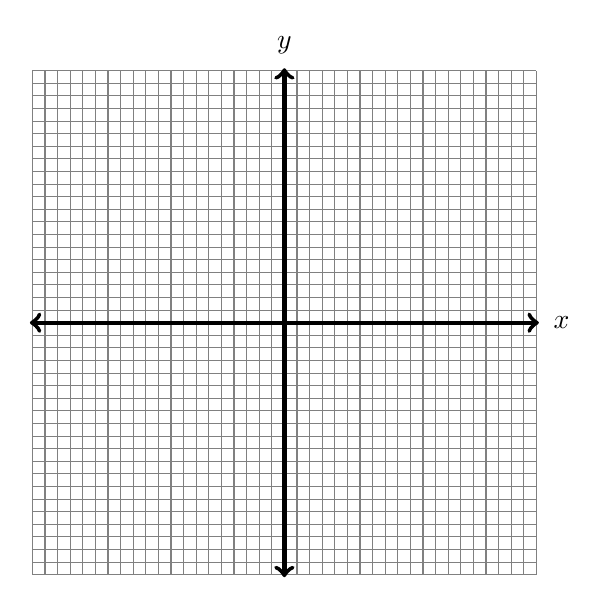
\begin{tikzpicture}[scale = 0.16]
      \draw[gray] (-20,-20) grid (20,20);
      \draw[ultra thick, <->] (-20.2,0)--(20.2,0);
      \draw[ultra thick, <->] (0,-20.2)--(0,20.2);
      \node at (22,0) {$x$};
      \node at (0,22) {$y$};
    \end{tikzpicture} ~~~
    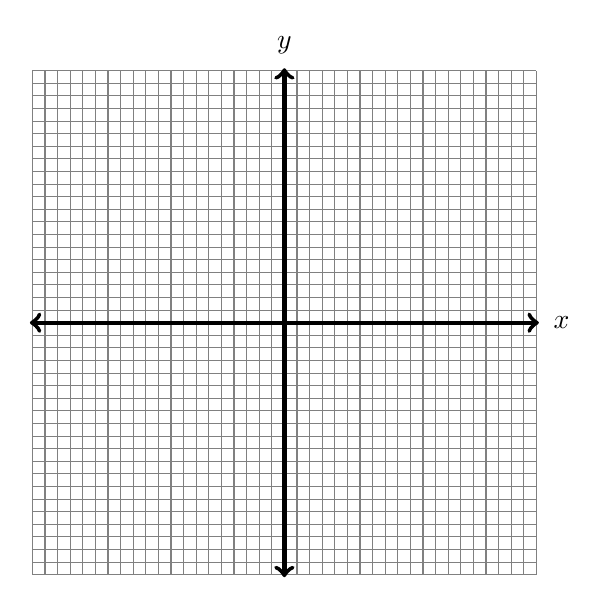
\begin{tikzpicture}[scale = 0.16]
      \draw[gray] (-20,-20) grid (20,20);
      \draw[ultra thick, <->] (-20.2,0)--(20.2,0);
      \draw[ultra thick, <->] (0,-20.2)--(0,20.2);
      \node at (22,0) {$x$};
      \node at (0,22) {$y$};
    \end{tikzpicture}
  \end{enumerate}
\end{document}
